\begin{pre}
	\thispagestyle{empty}
\begin{center}
  {\kaishu{材料来自于网上,如有侵权,请联系ocnzhao@163.com予以纠正,THX}}
\end{center}
\begin{center}
%		{\kaishu{人在春风和气中}}
\begin{figure}[htbp]
	\centering
	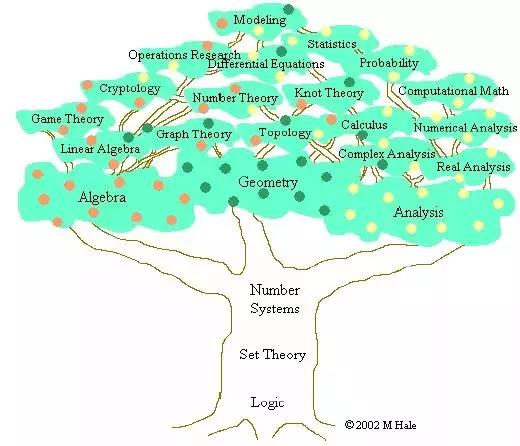
\includegraphics[width=0.5\textwidth]{Imagetreemath.png}
\end{figure}
\end{center}
\begin{center}
%		{\kaishu{人在春风和气中}}
\begin{figure}[htbp]
	\centering
	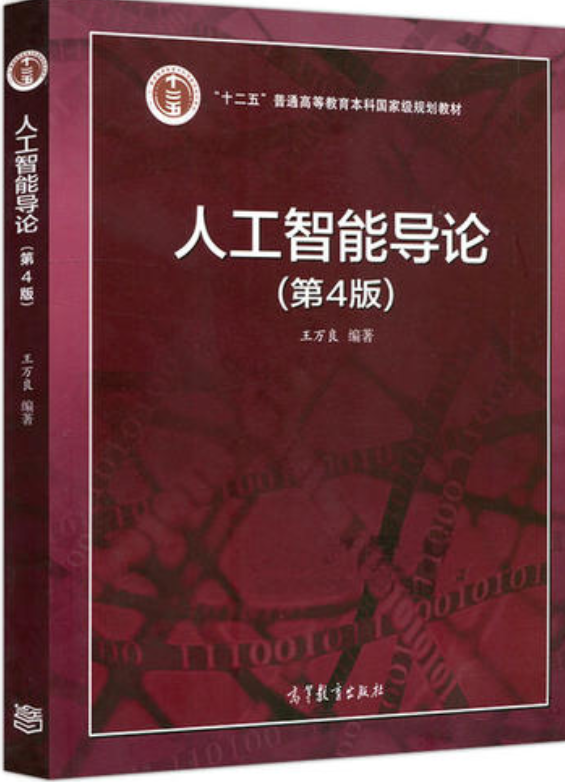
\includegraphics[width=0.46\textwidth]{ImageAIwwl01.png}
    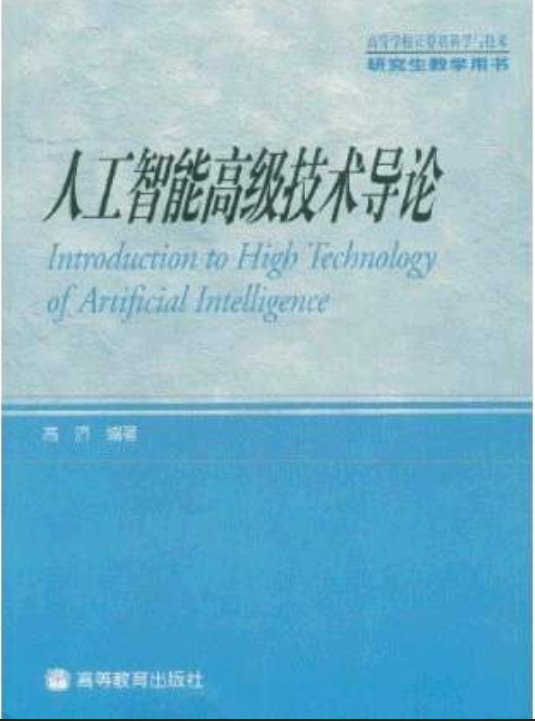
\includegraphics[width=0.45\textwidth]{ImageAIGQ.png}\\
    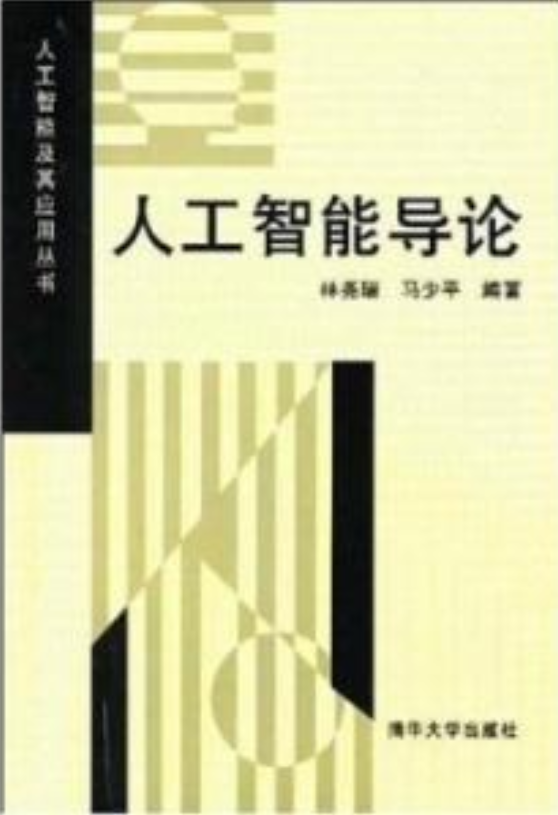
\includegraphics[width=0.45\textwidth]{ImageAILYR.png}
    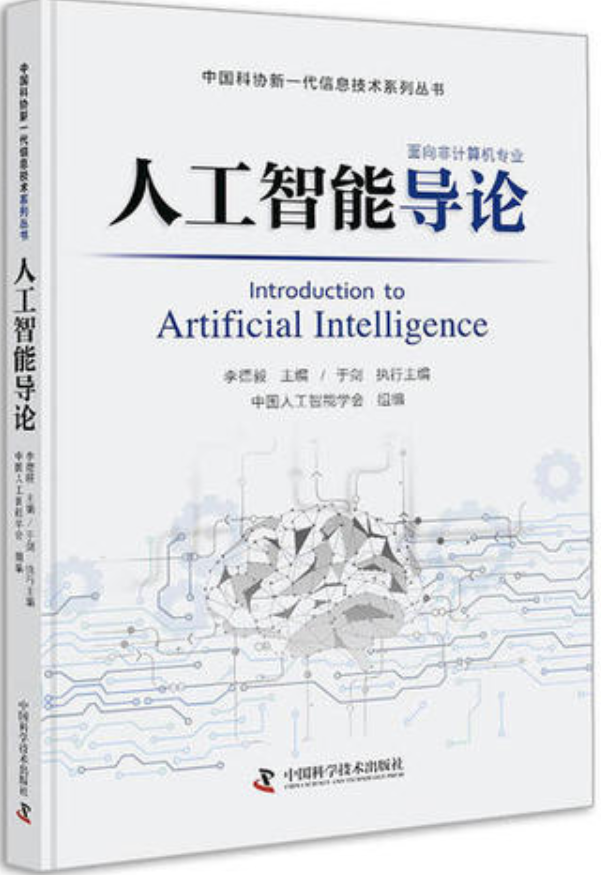
\includegraphics[width=0.45\textwidth]{ImageAILDY.png}\\
\end{figure}
\begin{figure}[htbp]
    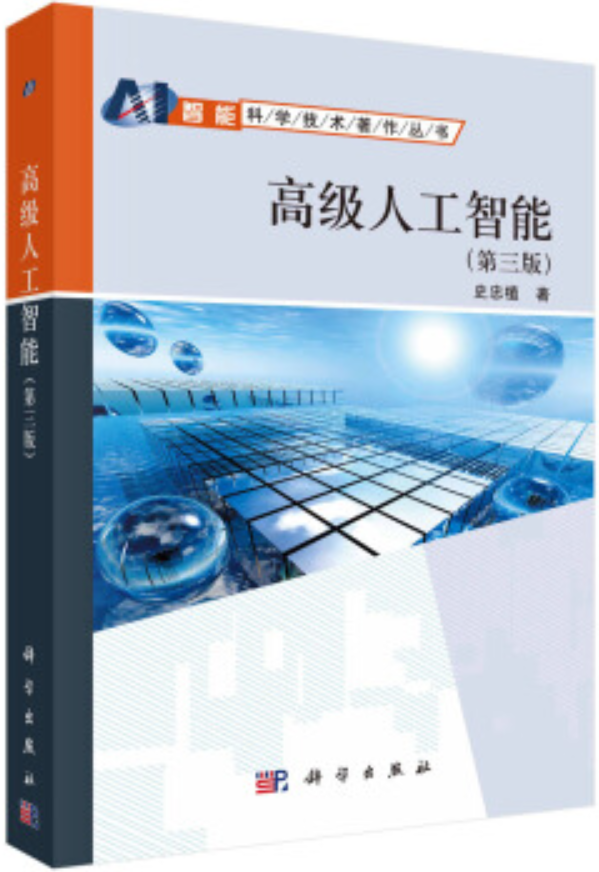
\includegraphics[width=0.45\textwidth]{ImageAISZZ.png}
    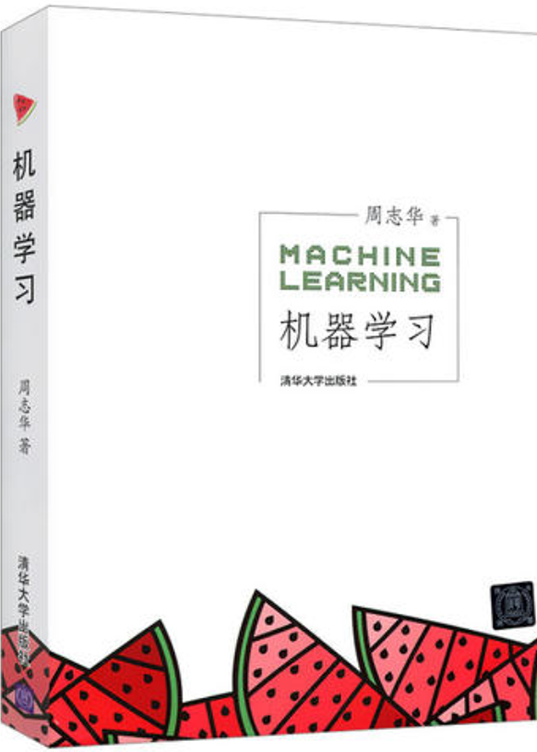
\includegraphics[width=0.45\textwidth]{ImageAIJQXX.png}
\end{figure}

史忠植——2013年凭借“拓展知识工程核心理论、创新分布智能理论基础、构建智能科学理论体系”成果, 荣获第三届吴文俊人工智能科学技术奖成就奖.

周志华——教育部“长江学者”特聘教授,国家杰出青年基金获得者;南京大学人工智能学院院长. 有一个旧称叫国立东南大学.
\end{center}

\href{https://www.sciencedaily.com/}{Science daily}
\paragraph{在线课程}

\href{https://ke.qq.com/webcourse/index.html?cid=1086628&term_id=101182654&lite=1&from=800021724#taid=5467185&vid=5285890799477964181}{人工智能基础-第一次}

\href{https://ke.qq.com/webcourse/index.html?cid=1086628&term_id=101182654&lite=1&from=800021724#taid=8423279&vid=5285890799803709554}{人工智能-研-第二次-发展和应用}

\href{https://edu.tipdm.org/notification?id=32302}{泰迪云课堂}

\href{http://speech.ee.ntu.edu.tw/~tlkagk/courses_ML20.html}{台大李宏毅老师的机器学习课程-2020}

\href{https://edu.tipdm.org/classroom/122/courses}{泰迪-深度学习原理及编程实现\_人邮版}

%\vspace*{5\baselineskip}
%\centerline{
\includegraphics[scale=0.6]{example/gzh.jpg}}
%\centerline{\fontsize{26pt}{26pt} 微信公众号}
\end{pre} 